\newlist{todolist}{itemize}{2}
\setlist[todolist]{label=$\square$}

\section*{Experiment protocol for investigators}

This protocol functions as a checklist for the investigators in the experiment "Using confidence levels of movement recognition in user training to improve prosthesis control". The checklist is used to ensure all steps in the experiment is performed correctly and that no steps will be neglected. The experiment consists of 3 session of 3-4 procedures in each session, as shown in \figref{fig:experiment_protocol_pipeline_investigators}. The same procedures (data acquisition, user training and performance test) occur in all sessions and needs to be performed similarly each session. A checklist for each procedure is described in the sections below \figref{fig:experiment_protocol_pipeline_investigators}.

\begin{figure}[H]                                         
	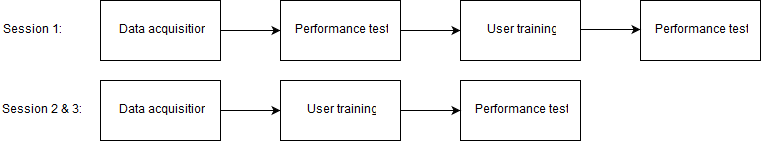
\includegraphics[width=0.9\textwidth]{figures/pMethods/experiment_protocol_pipeline}  
	\caption{Pipeline for the three sessions in the experiment and what procedures each session contains.}
	\label{fig:experiment_protocol_pipeline_investigators} 
\end{figure} 

The instruction of the of aim the respective procedures and content and functions in the interfaces is based on the information written in the experiment protocol for test subjects. (It is expected that the subject has read the experiment protocol handed out prior the experiment, but the information regarding the respective procedures is retold to verify that the subject has understood the following procedure.)

\textbf{\large Data acquisition}

\begin{todolist}
	\item Disinfect MYB with alco-swabs.
	\item Disinfect MYB application area of subject's dominant forearm with alco-swabs.
	\item Instruct subject to stand in anatomical standard position.
	\item Mark with a permanent marker the size of the main channel (channel with LED) of the MYB on the most lateral position of the thickest circumference of the subject's dominant forearm.
	\item Instruct subject in applying MYB with the main channel (channel with LED) located on the marked position. The MYB must be worn so that the LED is located as distally as possible. Add clips to tighten the MYB if necessary.
	\item Ensure that the main electrode-channel is placed correctly.
	\item Connect MYB in armband manager.
	\item Instruct subject in synchronizing MYB by performing extension until three distinct vibrations are felt. 
	\item Instruct subject in the movements about to be performed in the data acquisition.
	\item Instruct subject in performing an MVC; that the contraction must be steady during the 15 seconds.
	\item Record MVC for one movement. Observe spider plot meanwhile. If the activation pattern for the channels alters too much during the recording is to be discarded a new must be acquired.
	\begin{todolist}
		\item Extension
		\item Flexion
		\item Radial deviation
		\item Ulnar deviation
		\item Closed hand
		\item Opened hand
	\end{todolist}
	\item Instruct the subject in tracing the trapezoidal trajectory with the green cursor in different contraction levels of the MVC.
	\item Record contraction levels of MVC for one movement. Observe spider plot meanwhile. If the activation pattern for the channels alters too much during the recording is to be discarded a new must be acquired.
	\begin{todolist}
		\item Extension: $\square$ 40 \%, $\square$ 50 \%, $\square$ 60 \%
		\item Flexion: $\square$ 40 \%, $\square$ 50 \%, $\square$ 60 \%
		\item Radial deviation: $\square$ 40 \%, $\square$ 50 \%, $\square$ 60 \%
		\item Ulnar deviation: $\square$ 40 \%, $\square$ 50 \%, $\square$ 60 \%
		\item Closed hand: $\square$ 40 \%, $\square$ 50 \%, $\square$ 60 \%
		\item Opened hand: $\square$ 40 \%, $\square$ 50 \%, $\square$ 60 \%
	\end{todolist}
	\item Build regressors for each movement and build classifier trained with all movements.
\end{todolist}


\textbf{\large User training}

\begin{todolist}
	\item Instruct subject in aim of the user training, and explain the content and functions of the interface.
	\item Initiate user training.
\end{todolist}

\textbf{\large Performance test}

\begin{todolist}
	\item Instruct subject in aim of the performance test, and explain the content and functions of the interface.
	\item Initiate performance test.
	\item Save all training data and performance measures in folder named after name of subject, session number and which experiment group the subject belongs to.
\end{todolist}


